\section{Introduction}
\subsection{Background Gender Equality in Technology Sector}
\subsection{Background Low-Code /No-Code Development Platforms}
\subsection{Research Problem and Analytical Gap}
\subsection{Research Objectives and Questions}
\subsection{Structure of the Thesis}

Lorem Ipsum...

\begin{table}[!ht]
\centering
\begin{tabularx}{\textwidth}{|X|}
\hline
\multicolumn{1}{|c|}{\textbf{ Hypotheses}}\\ \hline
1. Hypo 1 \\ \hline
2. Hypo 2 \\ \hline
3. Hypo 3 \\ \hline
\end{tabularx}
\caption{Final Hypotheses}
\label{tab:hypo}
\end{table}

Table \ref{tab:hypo} shows the final hypotheses.

\begin{figure}[H]
\centering
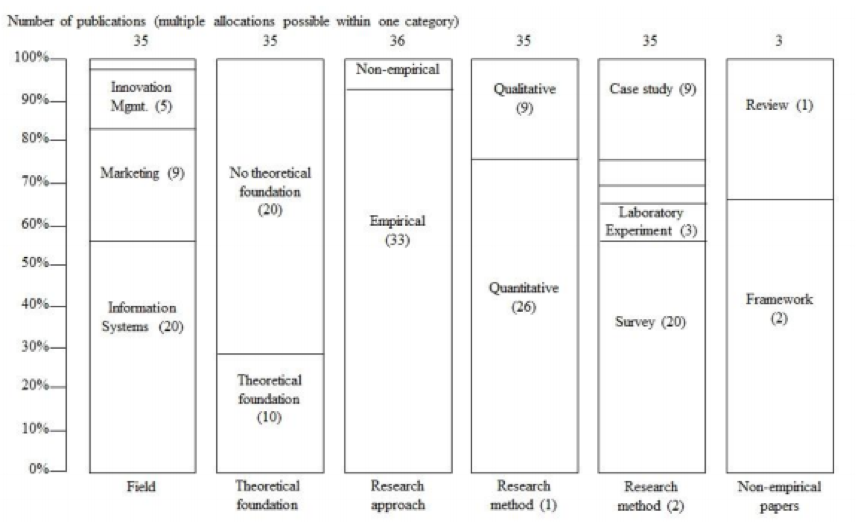
\includegraphics[width=1.0\textwidth]{images/Picture1.png}
\caption{Number of Publications} % \cite{teichert_machine_2019}}
\label{fig:nop}
\end{figure}

Figure \ref{fig:nop} shows the number of publications. 